\documentclass[a4paper]{article}

\usepackage{graphicx}

\usepackage{amsmath,amssymb}

\usepackage{minted}

\usepackage{multirow}

\usepackage{float}

\usepackage{todonotes}

\usepackage{forest}

\usepackage{xstring}

\usepackage{xcolor}

\usepackage[most]{tcolorbox}

\usepackage{xparse}

\usepackage{natbib}

\usetikzlibrary{graphs,graphdrawing}

\usegdlibrary{layered}

% for external graphviz

\input{/home/donkarlo/Dropbox/repo/nd_language_ai_project/src/nd_language_ai/formal/computer/programming/tex/latex/code_clips/external_graphviz.tex}

% for tags

\input{/home/donkarlo/Dropbox/repo/nd_language_ai_project/src/nd_language_ai/formal/computer/programming/tex/latex/part/control_sequence/kind/semtag/semtag.tex}

% for links

\input{/home/donkarlo/Dropbox/repo/nd_language_ai_project/src/nd_language_ai/formal/computer/programming/tex/latex/code_clips/seehere.tex}

\title{Neural cognitive architecture}

\date{}

\author{Mohammad Rahmani}

\begin{document}

   \label{neural_cognitive_architecture}
   In this section, the proposed architecture, together with its analogy to the biological human nervous system, is explained.

   \section{Agent’s architecture tree} The architecture is divided into the following sections.

      For a full agent architecture \seeherefooter{/nd_robotic_ai_learning_project/src/robot/part/psychophysiology_map.tex}

      \subsection{Body-mind dichotomy}
         \seeherefooter{/nd_robotic_ai_learning_project/src/robot/mind_body_transition/mind_body_problem.tex}
         The mind--body problem concerns the relationship between mental phenomena, such as thought and consciousness, and physical processes in the brain and body \cite{chambliss-2018-the-mind-body-problem}.

         In this research, this dichotomy is discussed and a bridge is proposed between the two.
      \subsection{Body}
         \subsubsection{Nervous system}

            \begin{figure}[H]
               \centering
               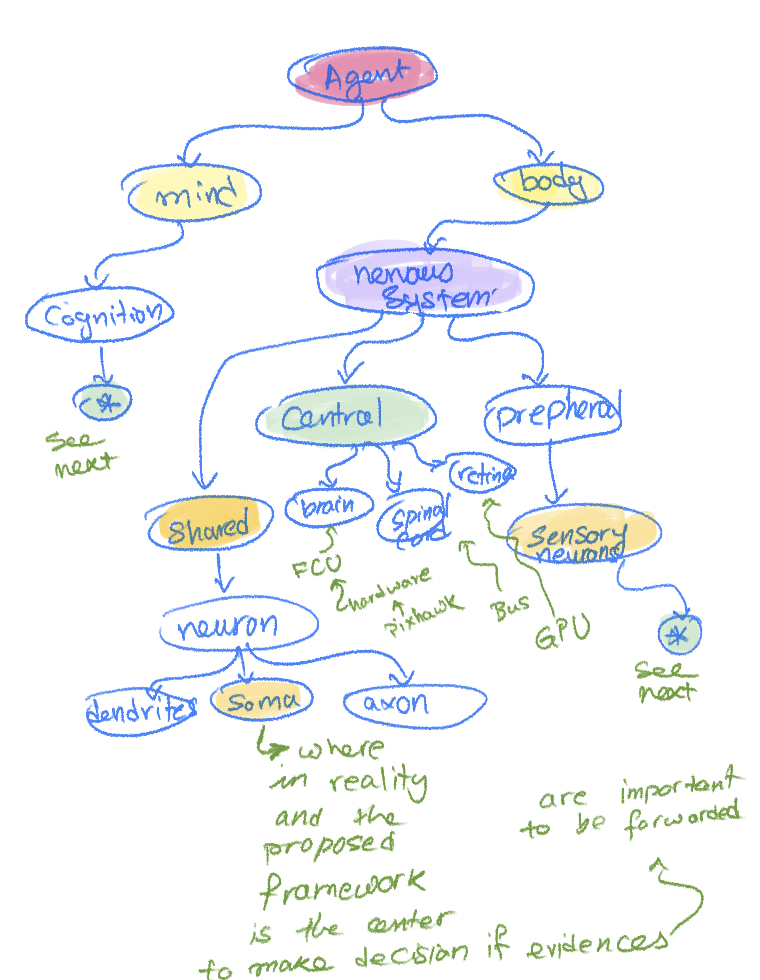
\includegraphics[width=0.9\textwidth]{physiopsycology.png}
            \end{figure}
      \subsection{Mind}
         \begin{figure}[H]
            \centering
            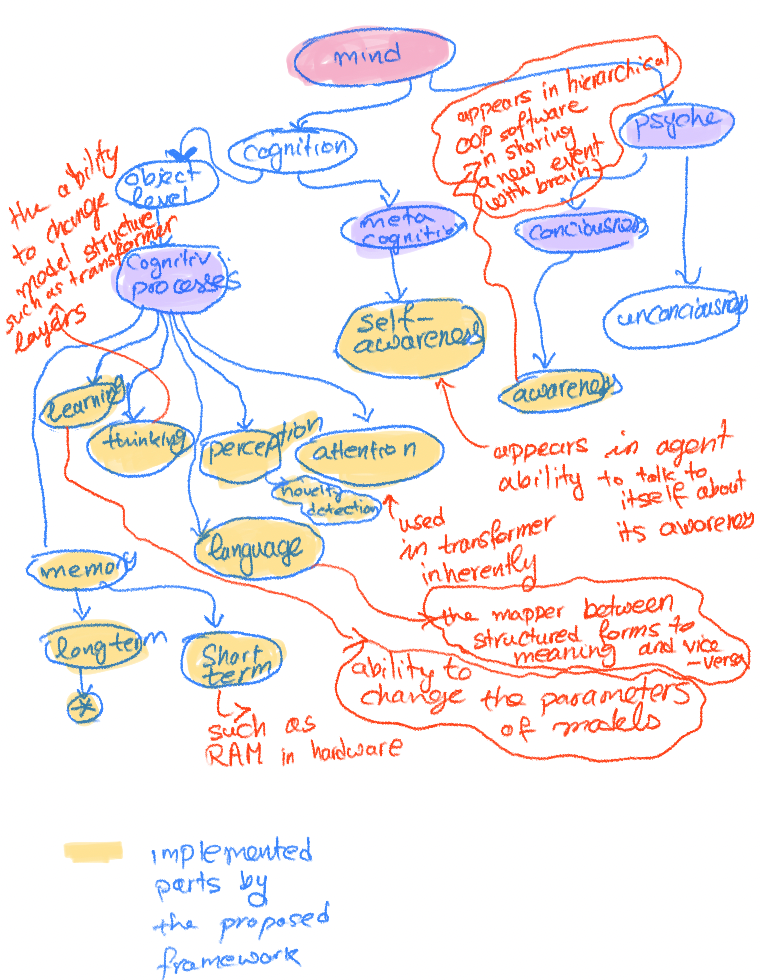
\includegraphics[width=0.9\textwidth]{mind_without_memory.png}
         \end{figure}
            \paragraph{Language} is a cognitive process that maps structured forms to meaning and meaning back to structured forms, independently of whether those forms are spoken, written, or signed \cite{matchin-2020-the-cortical-organization-of-syntax} \seeherefooter{/nd_robotic_ai_learning_project/src/robot/part/mind/cognition/part/object_level/process/part/language/language.tex}.
            \paragraph{Thinking} is the ability to change a model's structure, such as by changing the number of layers in a deep learning method \cite{markman-2001-thinking}.

               \begin{figure}[H]
                  \centering
                  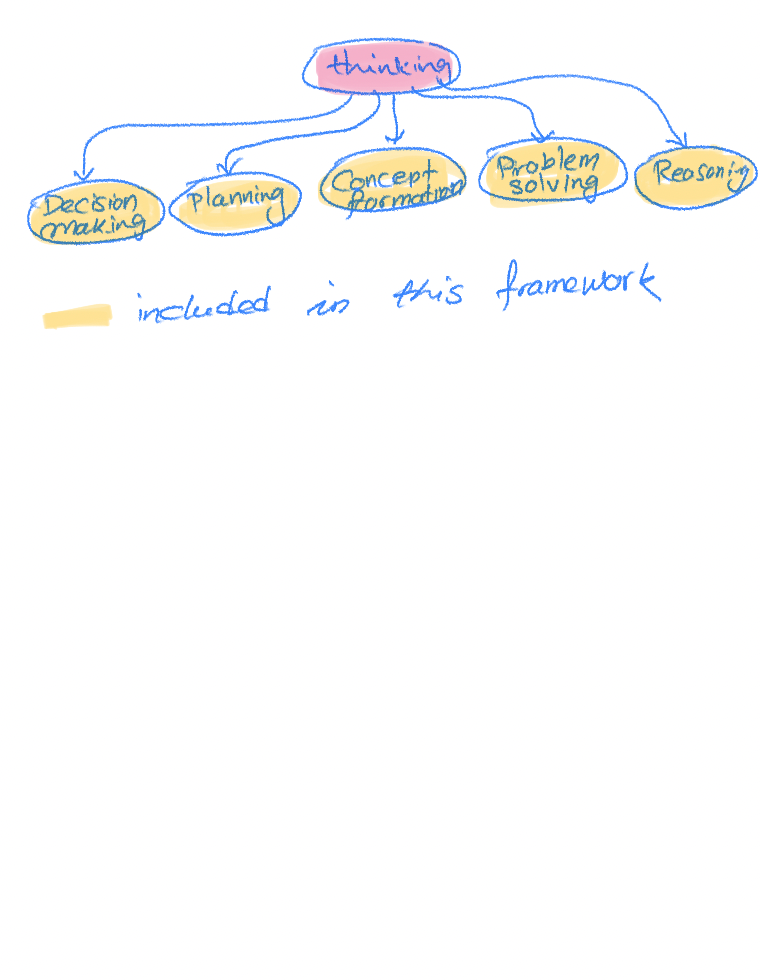
\includegraphics[width=0.9\textwidth]{thinking.png}
               \end{figure}

               In this research, although this hierarchy is not completely consistent with the literature, it is useful for understanding the proposed approach.
               \begin{figure}[H]
                  \centering
                  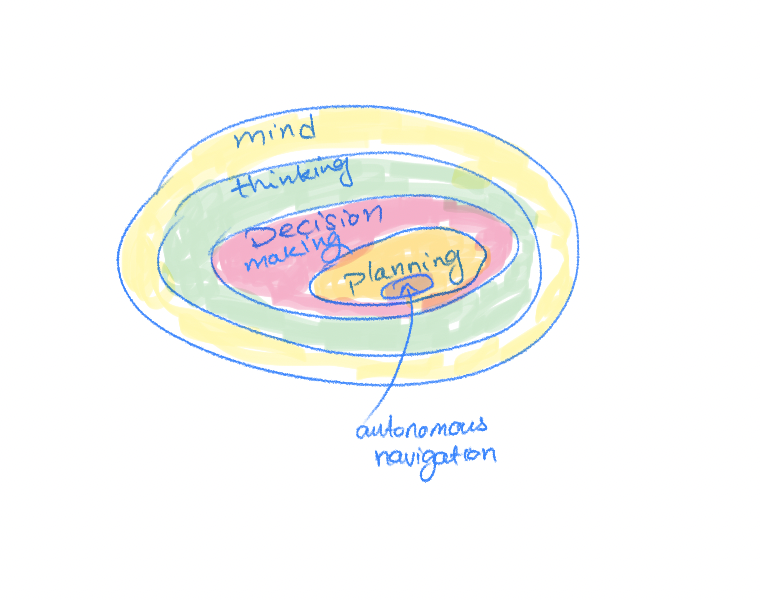
\includegraphics[width=0.9\textwidth]{thinking_van.png}
               \end{figure}
               \subparagraph{Decision making}
                  \seeherefooter{/nd_robotic_ai_learning_project/src/robot/part/mind/cognition/part/object_level/process/part/thinking/decision_making/decision_making.tex}
                  \cite{gold-2007-the-neural-basis-of-decision-making} argues that decision making is the cognitive process of deliberating over available information and committing to a choice.

                  In this research, decision making occurs during autonomous navigation while the agent attempts to minimize the level of surprise.

               \subparagraph{Planning}
                  \seeherefooter{/nd_robotic_ai_learning_project/src/robot/part/mind/cognition/part/object_level/process/part/thinking/planning/planning.tex}

                  \cite{mattar-2026-planning-in-the-brain-its-not-what-you-think-it-is} defines planning as the cognitive process of using internal simulations of possible future actions and states to guide behavior and learning.

                  In this research, planning occurs mainly during autonomous navigation through the minimization of surprise.
               \subparagraph{Concept formation}
                  \seeherefooter{/nd_robotic_ai_learning_project/src/robot/part/mind/cognition/part/object_level/process/part/concept_formation/concept_formation.tex}
                  \cite{sloutsky-2019-categories-concepts-and-conceptual-development}
                  describes concept formation as a cognitive process through which experience or language gives rise to conceptual categories that can subsequently be organized and used in higher-level cognition.


                  In this research, concept formation occurs during clustering and novelty detection.
               \subparagraph{Problem solving}
                  \seeherefooter{/nd_robotic_ai_learning_project/src/robot/part/mind/cognition/part/object_level/process/part/thinking/problem_solving/problem_solving.tex}

                  \cite{mayer-2013-problem-solving} describes problem solving as a cognitive processing directed toward achieving a goal when the method for reaching that goal is not initially known.

                  In this research, this ability is based on choosing actions to minimise surprise.

               \subparagraph{Reasoning}
                  \seeherefooter{/nd_robotic_ai_learning_project/src/robot/part/mind/cognition/part/object_level/process/part/thinking/reasoning/reasoning.tex}

                  \cite{johnson-laird-2010-mental-models-and-human-reasoning} argues that reasoning is the cognitive process of representing possibilities consistent with available information and deriving conclusions from those representations.

            \paragraph{Learning}
               \seeherefooter{/nd_robotic_ai_learning_project/src/robot/part/mind/cognition/part/object_level/process/part/learning/learning.tex}
               \cite{de-houwer-2013-what-is-learning-on-the-nature-and-merits-of-a-functional-definition-of-learning}
               Learning is the process of adaptation resulting from regularities in an organism's experience with its environment.

               In this research, learning occurs whenever model parameters are optimized, such as the weights of deep-learning methods including variational autoencoders or Transformers.
            \paragraph{Perception}
               \seeherefooter{/nd_robotic_ai_learning_project/src/robot/part/mind/cognition/part/object_level/process/part/perception/perception.tex}
               \cite{shin-2026-the-neural-code-of-perceptual-inference} defines perception as a process of inference in which incoming sensory evidence is interpreted based on prior expectations about the sensory world.

               In this research, this characteristic is realized by forming structured attribute--value data, referred to as a trace or engram, and then continuing the abstraction needed for language building and its use in state estimation.
            \paragraph{Attention}
               \seeherefooter{/nd_robotic_ai_learning_project/src/robot/part/mind/cognition/part/object_level/process/part/attention/attention.tex}
               \cite{chun-2011-a-taxonomy-of-external-and-internal-attention}
               Attention is the cognitive process of selecting, modulating, and sustaining focus on information that is most relevant for behavior.

               In this research, attention is used by multi-head attention-based Transformers to learn local sequential patterns in sequences.
         \subsubsection{Memory}
            Memory can be regarded as a neural property. However, in this research, for ease of presenting the method, it is treated as one of the cognitive processes of the mind, and a language is built for event-specific knowledge memory. Here is the taxonomy used for memory:

            \begin{figure}[H]
               \centering
               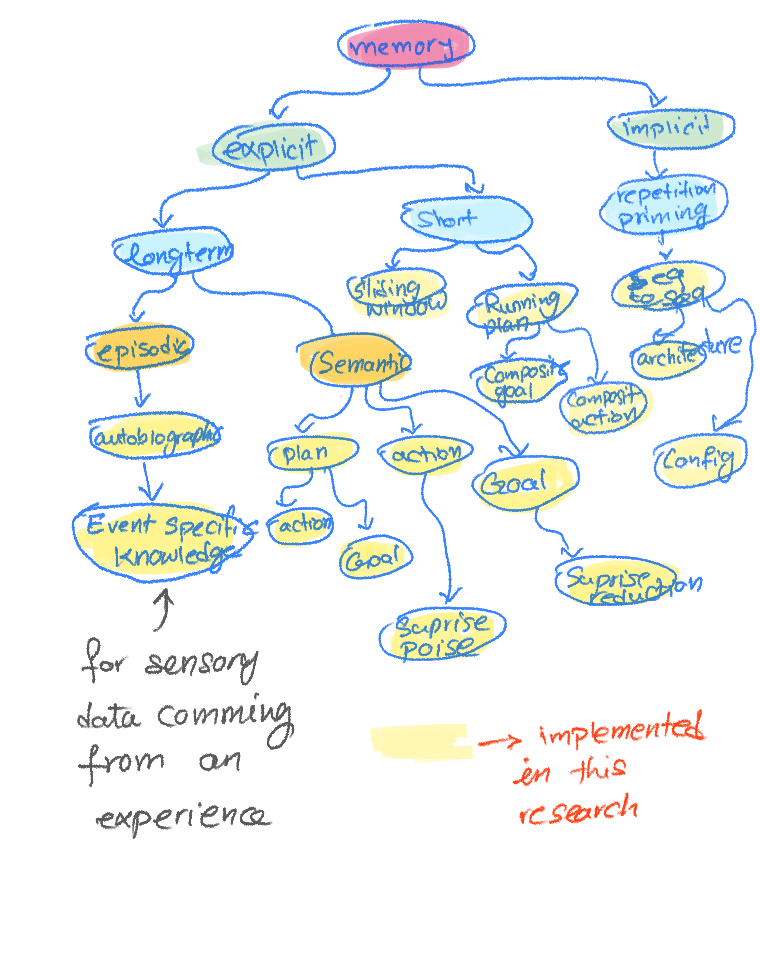
\includegraphics[width=0.9\textwidth]{memory.png}
            \end{figure}
            In this research, after guided learning, the agents are able to remember sensory data through their event-specific memory \cite{pillemer-2001-momentous-events-and-the-life-story}.

            This provides a biological analogy for mental time travel \seeherefooter{/nd_robotic_ai_learning_project/src/robot/part/mind/cognition/part/object_level/process/part/thinking/planning/mental_time_travel.tex}, allowing the past to be remembered chronologically.

   \section{Architecture ontology}
      \begin{figure}[H]
         \centering
         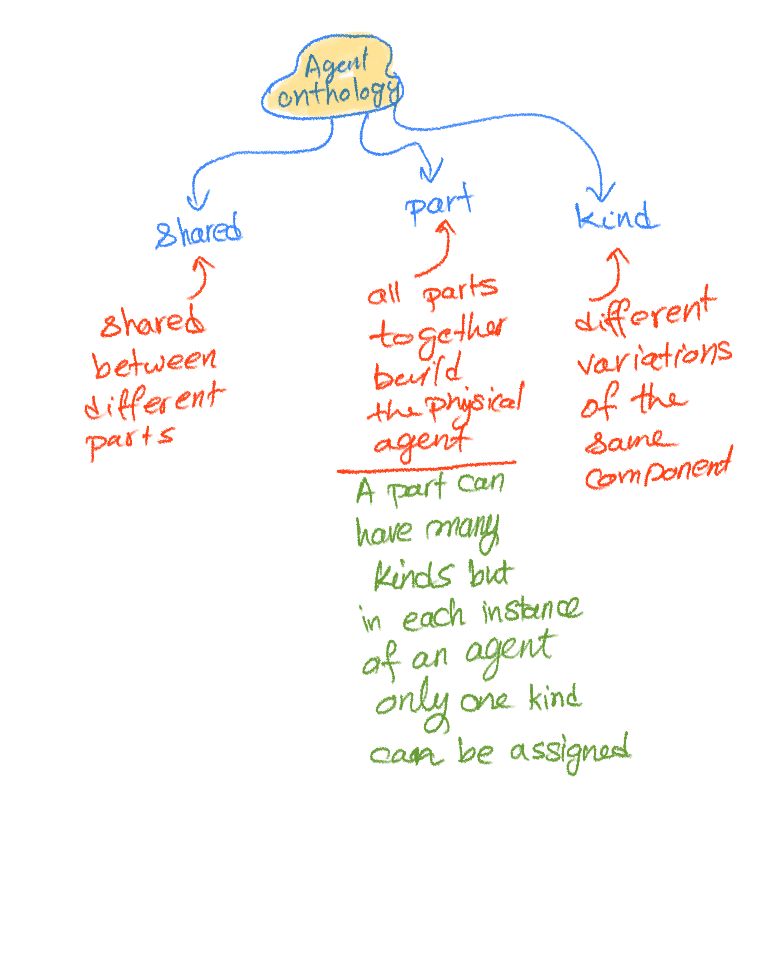
\includegraphics[width=0.9\textwidth]{agent_onthology.png}
      \end{figure}
      \subsection{Engram or trace}
         \seeherefooter{/nd_robotic_ai_learning_project/src/robot/part/mind/cognition/part/object_level/process/part/memory/part/shared/engram/engram.tex}

         An engram refers to a unit of cognitive information encoded in a physical medium. It is hypothesized to represent the mechanism through which memories are preserved as biophysical or biochemical modifications in the brain or other biological tissues following external stimulation \cite{josselyn-2020-memory-engrams-recalling-the-past-and-imagining-the-future,sakaguchi-2012-catching-the-engram-strategies-to-examine-the-memory-trace}.

         In this research, a trace is considered a labeled data point or an attribute--value data point, linguistically equivalent to a feature structure \cite{kay-1984-functional-unification-grammar, kasper-1986-a-logical-semantics-for-feature-structures} \seeherefooter{/nd_robotic_ai_learning_project/src/robot/part/mind/cognition/part/object_level/process/part/language/theory/universal_grammar/part/feature_structure/feature_structure.tex}

   \section{Nervous system}
      The architecture should be considered a brain composed of neurons and formulated as probabilistic graphical models.

      Each neuron receives a set of evidence and weights it according to what it learned during the learning-by-demonstration phase described in \ref{methodology_neural_encoder_tarining}, and finally decides whether to spike. If it does, an action potential propagates evidence to the next vertical or horizontal neuronal layers. This weighting and spiking process continues until the brain determines the probability distribution at each vertical state.

      During training and anomaly detection, specific neurons may appear that are activated only in those phases.

      In this section, we explain only the architecture shared between the two aforementioned phases. First, a brief explanation of the neuron and its spiking mechanism is provided.

   \section{Anatomy of a neuron}

      A neuron is composed of

      \begin{itemize}
         \item Soma/Cell body (evidence potential weighting center)
         \begin{itemize}
            \item Membrane potential
            \begin{itemize}
               \item Graded potential
            \end{itemize}
         \end{itemize}
         \item Axons and their terminals (output)
         \item Dendrites (inputs)
      \end{itemize}

      \begin{figure}[H]

         \centering

         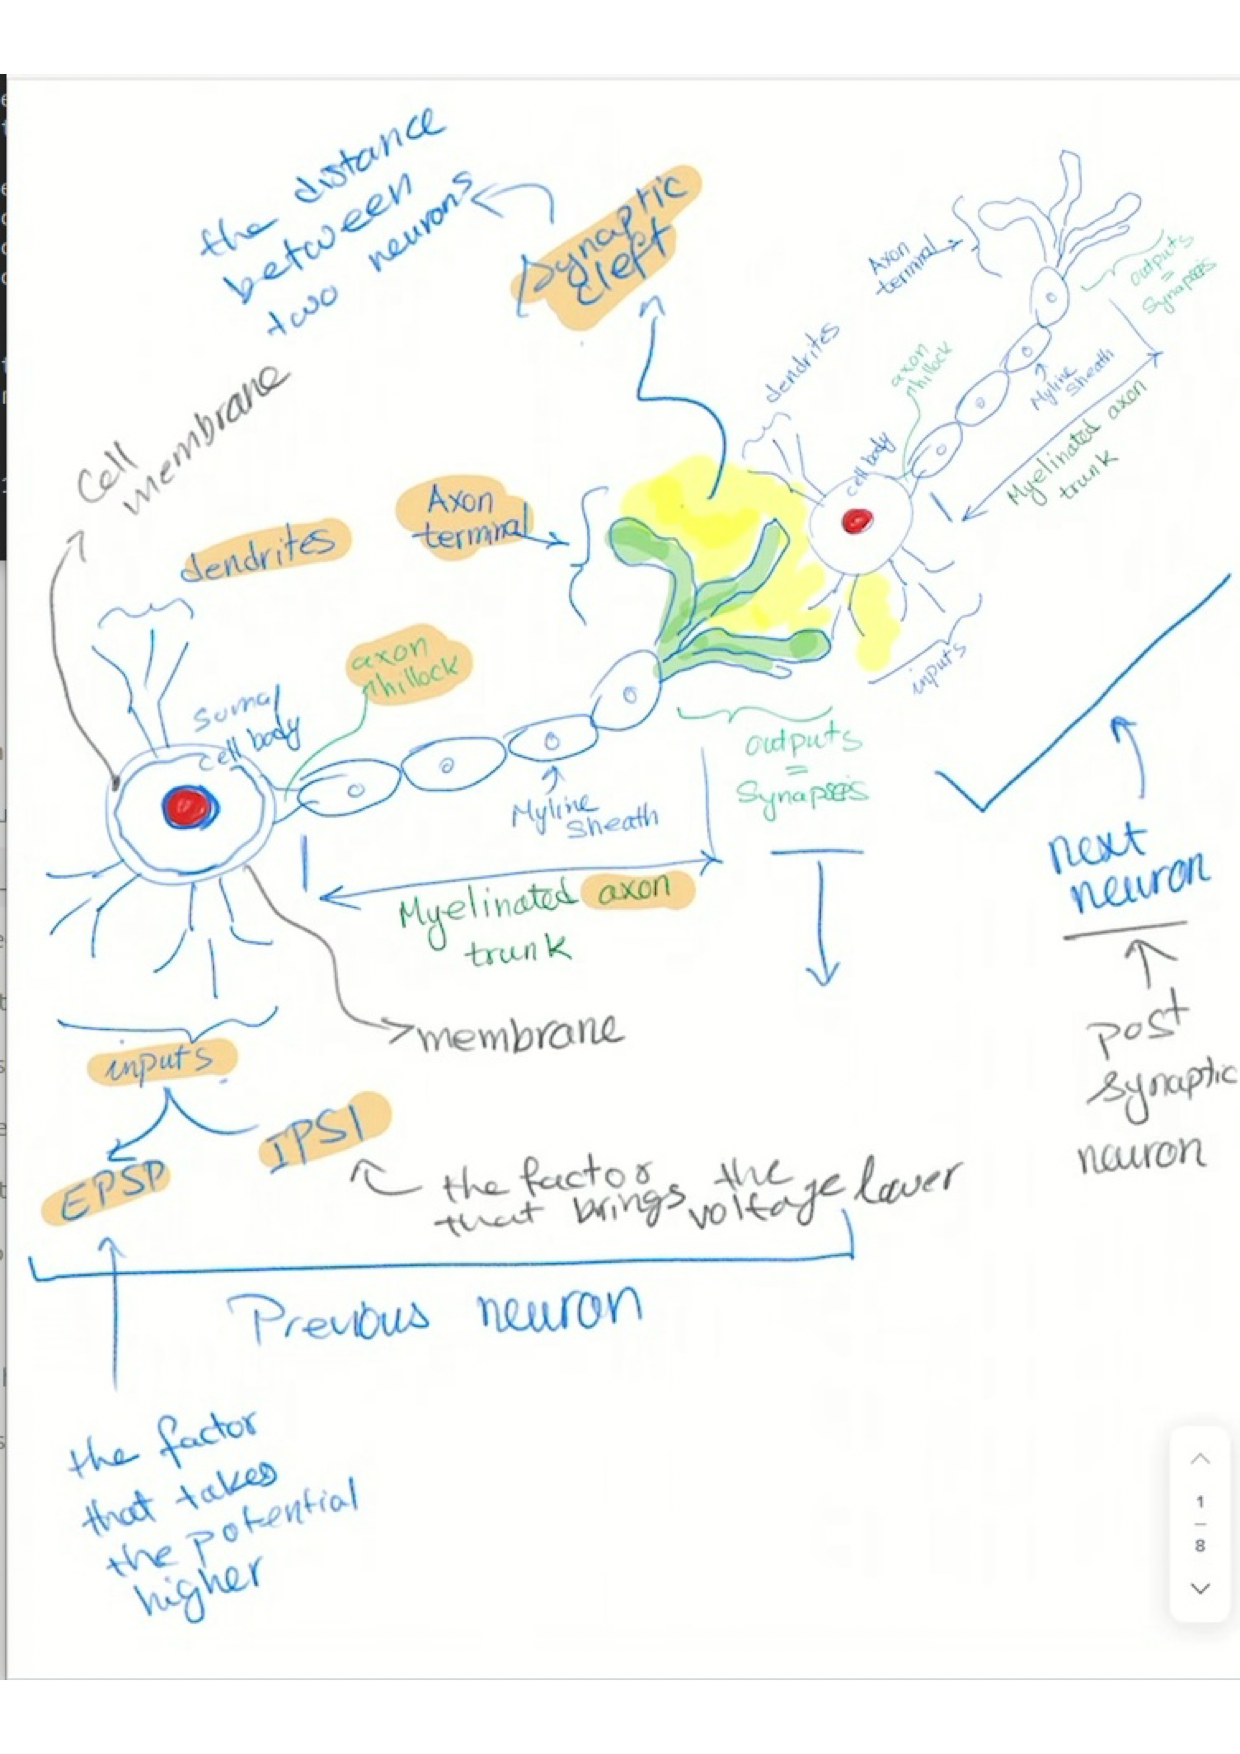
\includegraphics[width=0.9\textwidth]{neuron.png}

      \end{figure}

      \subsection{Graded potentials}

         \begin{itemize}
            \item IPSP (to decrease the evidence potential)
            \item EPSP (to increase the evidence potential)
         \end{itemize}

      \subsection{Anatomy of action potentials}

         The decision to spike or not is one of the most basic yet fundamental decisions made in the human body. \iffalse I remember there was a paper mentioning this \fi. Later, we will see that this research extends this dichotomy to more complex language abstractions. In this research, the shape of an action potential, as well as its temporal firing pattern, carries information. This also occurs biologically because the action-potential waveform is not identical across neuronal types; sensory-neuron subtypes can exhibit characteristic differences in action-potential duration, overshoot, repolarization profile, and afterhyperpolarization \cite{korner-2022-functional-subgroups-of-rat-and-human-sensory-neurons-a-systematic-review-of-electrophysiological-properties}.
         \begin{figure}[H]

            \centering

            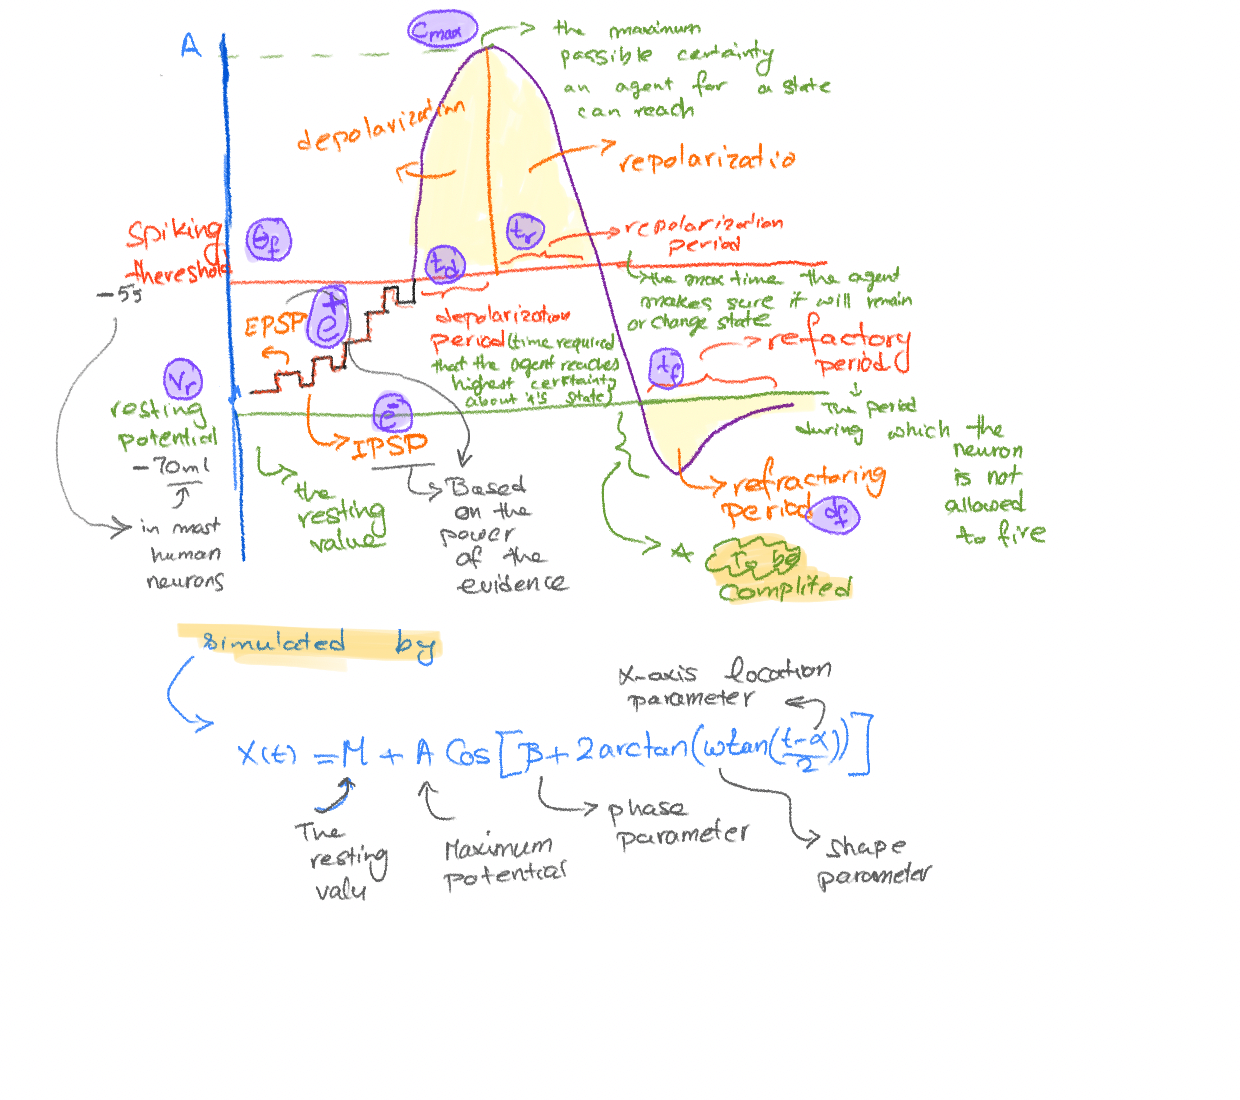
\includegraphics[width=0.9\textwidth]{action_potential_anatomy.png}

         \end{figure}


         \begin{itemize}
            \item \textbf{Depolarization period}
            \begin{itemize}
               \item The time required after the neuron starts firing to obtain sufficient confidence that the agent is, with the highest probability, in the represented state.
               \item Learned peak of action-potential depolarization. This parameter shows the maximum certainty that the state neuron could reach during training. The highest value is 1 and the lowest is 0.
            \end{itemize}
            \item \textbf{Repolarization period}
            \begin{itemize}
               \item The time required to obtain sufficient confidence that the agent has either remained in the same state with approximately constant intensity or transitioned to a different state.
               \item Learned firing tolerance (in some biological neurons, it is -70). This parameter indicates the point at which there is sufficient certainty that the agent is in that state, causing the state neuron to spike.
            \end{itemize}
            \item \textbf{Refractory period} (during which, even if enough evidence exists for another spike, the neuron cannot spike). With each spike, the accumulated evidence is cleared and the system returns to its resting potential.
            \begin{itemize}
               \item The time period during which the neuron is not allowed to fire again, even if the accumulated EPSPs are sufficient to overcome the IPSPs and cross the firing threshold.
               \item \textbf{Refractory duration:} the time interval after a spike during which the state neuron is not allowed to fire again, even if sufficient evidence is accumulated.
               \item \textbf{Refractory depth:} the strength of the post-spike inhibition or reset applied to the neuron's evidence potential. A larger refractory depth requires stronger subsequent evidence before the neuron can reach the firing threshold again.
            \end{itemize}
            \item \textbf{The resting membrane potential:} value (in some biological neurons, it is -50). It is the average amount of evidence/potential (IPSP, EPSP) that the state neuron has while the agent is not in that state. It represents prior or baseline evidence that usually exists in the state neuron.
         \end{itemize}

         \subsubsection{Simulation with ``Frequency-Modulated Möbius (FMM)``}

            \seeherefooter{/nd_robotic_ai_learning_project/src/robot/part/body/part/nervous_system/part/shared/neuron/part/action_potential/wave_form/kind/frequency_modulated_mobius/frequency_modulated_mobius.tex}

            \begin{equation}
               X(t)
               =
               M
               +
               A
               \cos
               \Biggl[
               \beta
               +
               2
               \arctan
               \Biggl(
               \omega
               \tan
               \Bigl(
               \frac{t-\alpha}{2}
               \Bigr)
               \Biggr)
               \Biggr]
            \end{equation}

            \begin{itemize}
               \item $X(t)$ is the value of the FMM wave at time $t$.

               \item $M$ is the baseline parameter. Bound: $M \in \mathbb{R}$.
               It controls the vertical shift of the FMM signal without changing
               the waveform shape, phase, or temporal deformation.

               \item $t$ is time. Bound: $t \in [0, 2\pi)$.

               \item $A$ is the amplitude parameter. Bound: $A \geq 0$.
               It controls the vertical scale of the waveform.

               \item $\alpha$ is the location parameter. Bound:
               $\alpha \in [0, 2\pi)$. It controls the horizontal position of
               the waveform on the time axis.

               \item $\beta$ is the phase parameter. Bound:
               $\beta \in [0, 2\pi)$. It controls the internal phase of the wave.
               Together with $\alpha$ and $\omega$, it determines the temporal
               position of the maximum and minimum points of the waveform.

               \item $\omega$ is the shape parameter. Bound:
               $\omega \in (0, 1]$. It controls the sharpness, skewness, and
               temporal deformation of the waveform. When $\omega$ is close to
               zero, the waveform becomes more spike-like; when $\omega$ is close
               to one, the waveform becomes more similar to a sinusoidal wave.
            \end{itemize}
      \subsection{Spike trains}
         \seeherefooter{/nd_robotic_ai_learning_project/src/robot/part/body/part/nervous_system/part/shared/neuron/part/action_potential/train.tex}
         A temporal sequence of action potentials generated by a neuron is called its ``spike train``. The more densely a neuron spikes within a given time interval, the higher the value of that sensor is.
         \cite{vandrongelen-2007-spike-train-analysis}

         This research uses APT to represent a spike train.


   \section{Neuron types}

      \subsection{Sensory - receptors}

         In the human body, the sensory neuron and receptor are sometimes the same and sometimes separate. In this research, for the sake of simplicity, they are treated as the same. Although a sensory receptor in the human body is responsible for converting a stimulus into electrical signals and then passing them to a sensory neuron to generate action potentials, this research considers these two stages to occur in a single neuron.

         \begin{figure}[H]

            \centering

            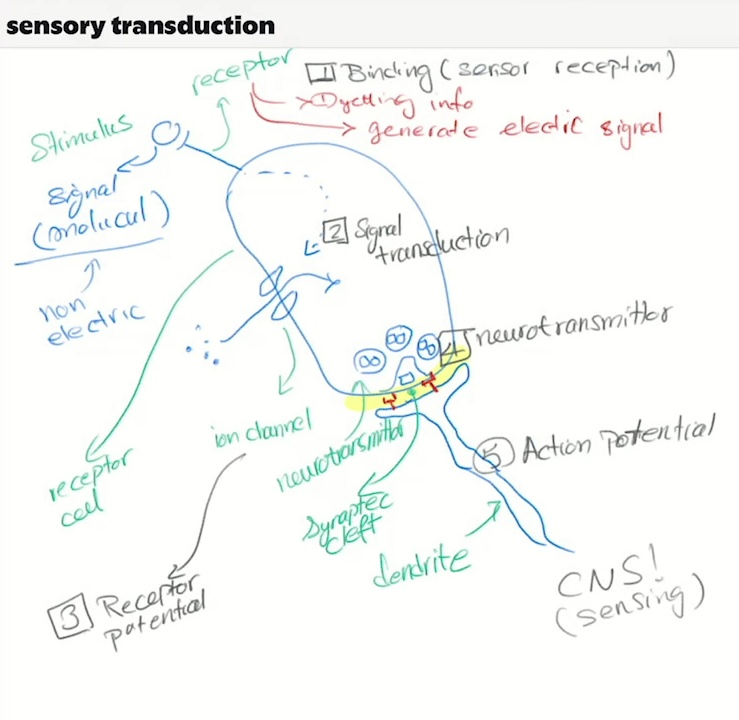
\includegraphics[width=0.9\textwidth]{sensory_transduction.png}

         \end{figure}


         Simplified sensory transduction

         \begin{figure}[H]
            \centering
            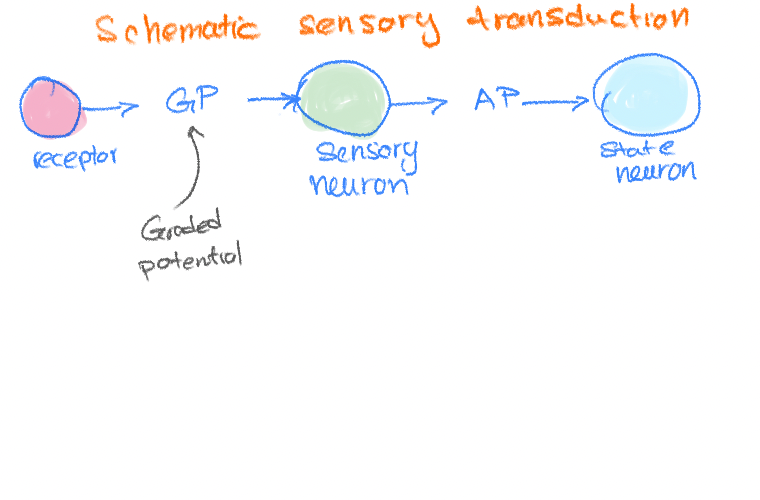
\includegraphics[width=0.9\textwidth]{sensory_transduction_schematic.png}
         \end{figure}

   \section{Neural population}
      \subsection{Neural circuits}
         A neural circuit consists of interconnected neurons whose synaptic interactions enable them to perform a particular function. Individual neural circuits can also interact with other circuits, forming larger-scale networks across the brain. \seeherefooter{/nd_robotic_ai_learning_project/src/robot/part/body/part/nervous_system/part/shared/neuron/population/kind/network/shared/circuit/circuit.tex}
         \subsubsection{Intensity and intensity-change-rate neurons}
            In most cases, two types of sensory neurons work together. One fires continuously as long as the stimulus exists and fires more when the intensity of the stimulus increases. The other fires more when the rate of change of the stimulus increases. For example, in vision, sustained retinal ganglion cells fire more when light intensity increases, while transient retinal ganglion cells fire more when the rate of change of light intensity increases.
            \begin{figure}[H]
               \centering
               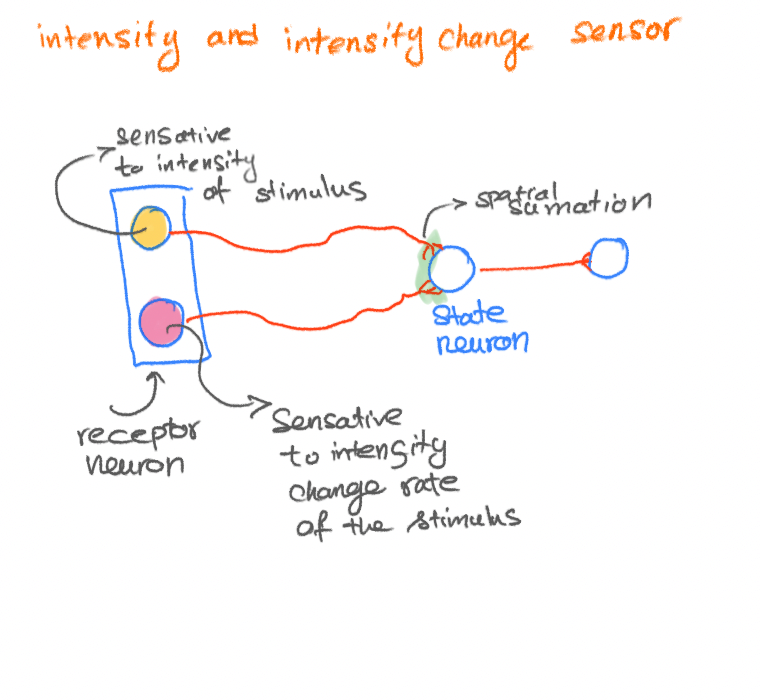
\includegraphics[width=0.9\textwidth]{intensity_and_intensity_rate_change.png}
            \end{figure}


         \subsubsection{Different types of potential summation in a destination neuron}
            \begin{figure}[H]
               \centering
               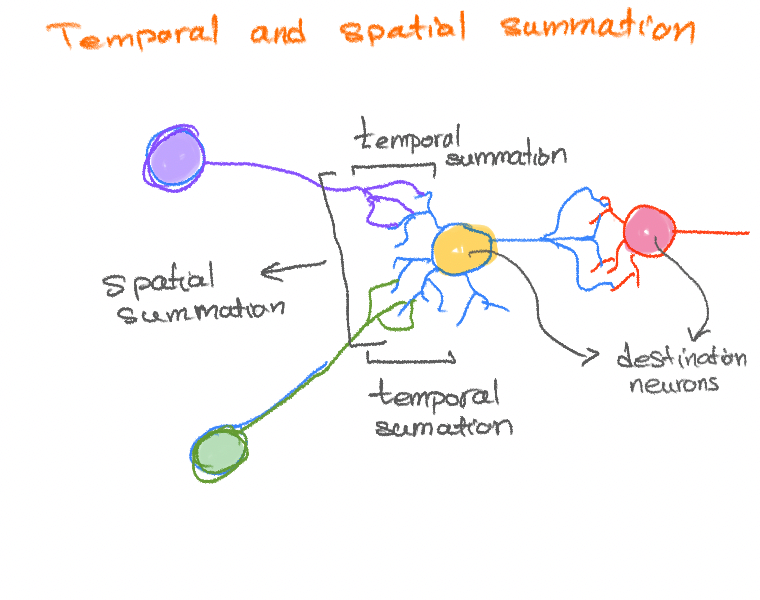
\includegraphics[width=0.9\textwidth]{temporal_and_spacial_summation.png}
            \end{figure}
            \paragraph{Spatial summation}
               Summation of potentials coming from different neurons.
            \paragraph{Temporal summation}
               Summation of the potentials from one spike train.


      \subsection{Neural pool and the whole architecture together}
         Neuronal pools are groups of interconnected neurons organized to receive, integrate, and transmit neural signals in characteristic ways \cite{brainkart-2017-transmission-and-processing-of-signals-in-neuronal-pools}.
         \subsubsection{Population coding}

            \cite{shimazaki-2025-neural-coding-foundational-concepts-statistical-formulations-and-recent-advances} emphasizes that neural information is often represented at the population level, where

            \begin{itemize}
               \item firing rate
               \item temporal structure
               \item correlations between neurons
            \end{itemize}
            jointly affect how accurately stimuli can be encoded and decoded.


            \begin{figure}[H]
               \centering
               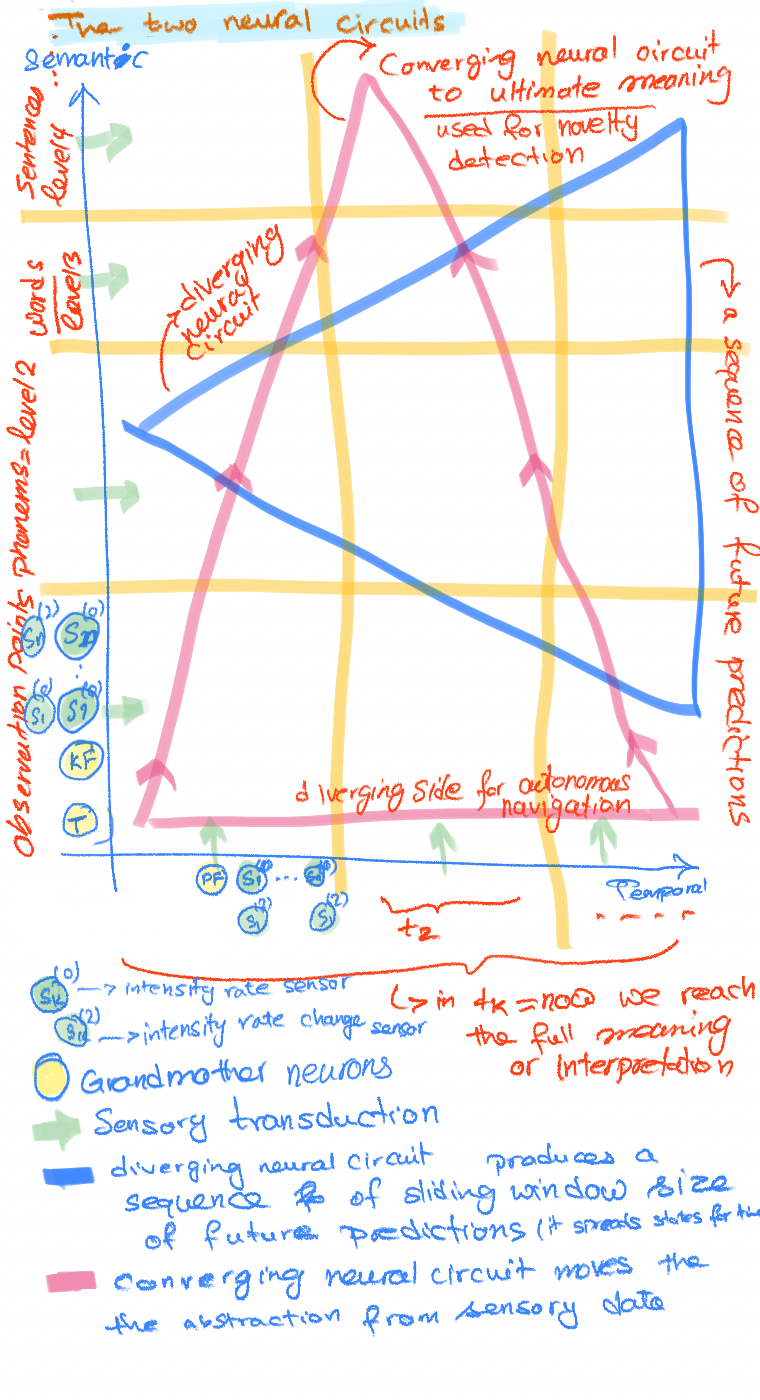
\includegraphics[width=0.9\textwidth]{neural_pool.png}
            \end{figure}
         
      \subsection{Large scale brain networks}
         This research does not discuss or implement large-scale brain networks. It only argues, where necessary, that the approach taken to build computational MRS self-awareness is biologically plausible. Therefore, only a short introduction to three of the most important networks is provided here.
         \begin{figure}[H]
            \centering
            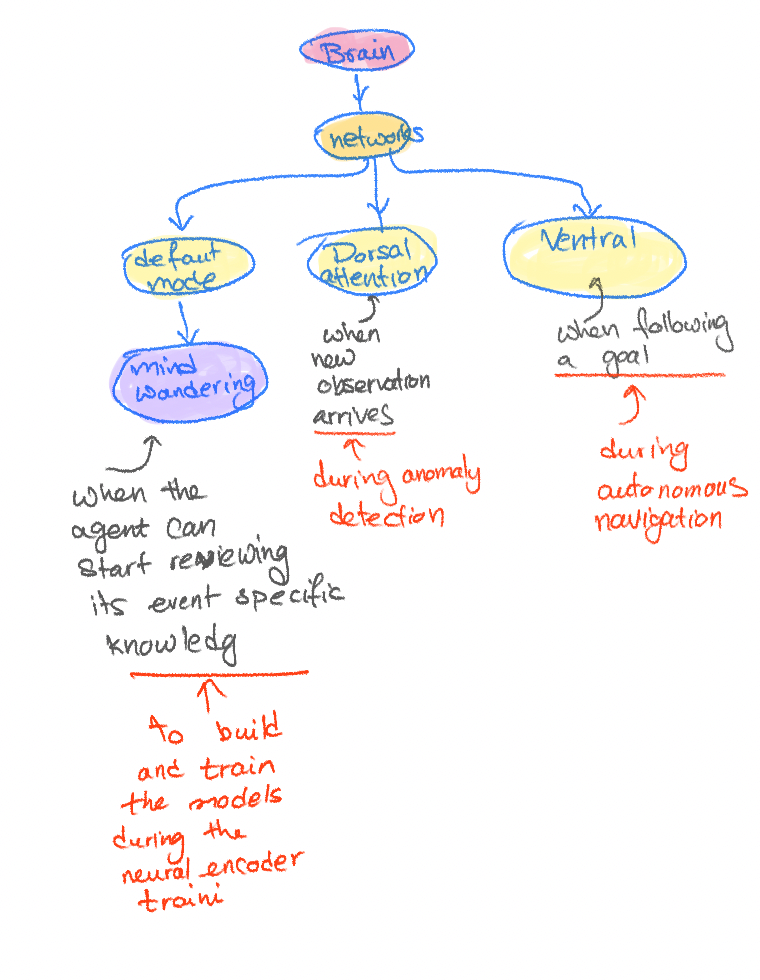
\includegraphics[width=0.9\textwidth]{large_scale_barin_networks.png}
         \end{figure}
         \subsubsection{Default mode/mind wandering}
            The default mode network is primarily active during internally directed cognition, such as mind wandering, autobiographical memory, and self-referential thought  \cite{mason-2007-wandering-minds-the-default-network-and-stimulus-independent-thought}.

         \subsubsection{Dorsal attention}
            The dorsal attention network supports voluntary, goal-directed (top-down) attention by selecting and maintaining focus on task-relevant information \cite{corbetta-2002-control-of-goal-directed-and-stimulus-driven-attention-in-the-brain, vossel-2014-dorsal-and-ventral-attention-systems, corbetta-2008-the-reorienting-system-of-the-human-brain-from-environment-to-theory-of-mind}.

         \subsubsection{Ventral attention}
            The ventral attention network detects salient or unexpected stimuli and reorients attention toward them in a stimulus-driven (bottom-up) manner \cite{scalf-2014-trial-history-effects-in-the-ventral-attentional-network}.

            \include{/nd_research_publication/src/kind/journal_2026/methodology/part/neural_cognitive_architecture/language.tex}
            
            \include{/nd_research_publication/src/kind/journal_2026/methodology/part/neural_cognitive_architecture/prediction_and_state_estimation_model/prediction_and_state_estimation_model.tex}

            \bibliographystyle{plainnat}

            \bibliography{/nd_shared_research/bibliography/bibliography.bib}

\end{document}
